\section{Experimental Evaluation and Discussion}\label{sec:experiments}

\subsection{Experimental Setup}
\subsubsection{Dataset and Partitioning}
To comprehensively evaluate multimodal task performance, we conduct evaluations on the Task-Directed Image Understanding and Challenge (TDIUC) benchmark~\cite{kafle2017tdiuc}, one of the most rigorous and diverse VQA datasets designed to measure specific reasoning capabilities while mitigating language bias. 

The evaluation encompasses 2,400 independent blind test images across six representative semantic task categories (400 images per category):
\begin{enumerate}
    \item \textbf{Object Presence}: Binary verification of object existence within the scene.
    \item \textbf{Counting}: Enumeration of target objects requiring fine-grained spatial localisation.
    \item \textbf{Positional Reasoning}: Determining relative spatial configurations (e.g., ``to the left of'', ``behind'').
    \item \textbf{Scene Recognition}: Identifying overall environmental context (e.g., kitchen, highway, runway).
    \item \textbf{Activity Recognition}: Classifying human or vehicular action dynamics.
    \item \textbf{Color Recognition}: Discriminating object chromatic attributes under varying illumination.
\end{enumerate}
The policy training set contains 4,800 images, and the validation set comprises 1,200 images. Strict image-hash deduplication ensures zero overlap across training, validation, and test splits.

\subsubsection{Physical Layer and Wireless Channel Simulation}
Wireless channels are simulated across 10 channel SNR operating points:
\begin{equation}
\gamma \in \{-5.0, -2.5, 0.0, 2.5, 5.0, 7.5, 10.0, 12.5, 15.0, 20.0\}\text{ dB}.
\end{equation}
The channel undergoes block flat Rician fading with a Rice factor $K = 6\text{ dB}$. Channel coding is performed via a 3GPP 5G-compliant $\text{LDPC}(1020, 512)$ code with QPSK digital modulation ($m=2$). The receiver executes iterative Soft Belief Propagation (BP) decoding up to 50 iterations with early termination based on parity-check equations, followed by CRC-32 cyclic redundancy verification.

\subsubsection{Model and Computational Hardware Specifications}
Neural image source compression is implemented via the CompressAI \texttt{bmshj2018-hyperprior} variational architecture. The edge VLM is Qwen3-VL-4B-Instruct, loaded in 4-bit NormalFloat (NF4) quantization and adapted via rank-8 LoRA on the language backbone attention projections ($5{,}898{,}240$ trainable parameters). 

Inference latency and energy benchmarks are profiled on an enterprise-grade computing platform equipped with an NVIDIA A100 Tensor Core GPU (80GB VRAM, PCIe Gen4, TDP 300W) and an AMD EPYC 7763 64-Core Processor. GPU power is recorded via NVML hardware monitoring, and forward inference latency is measured with microsecond CUDA synchronization events after GPU warmup.

\begin{figure*}[!t]
\centering
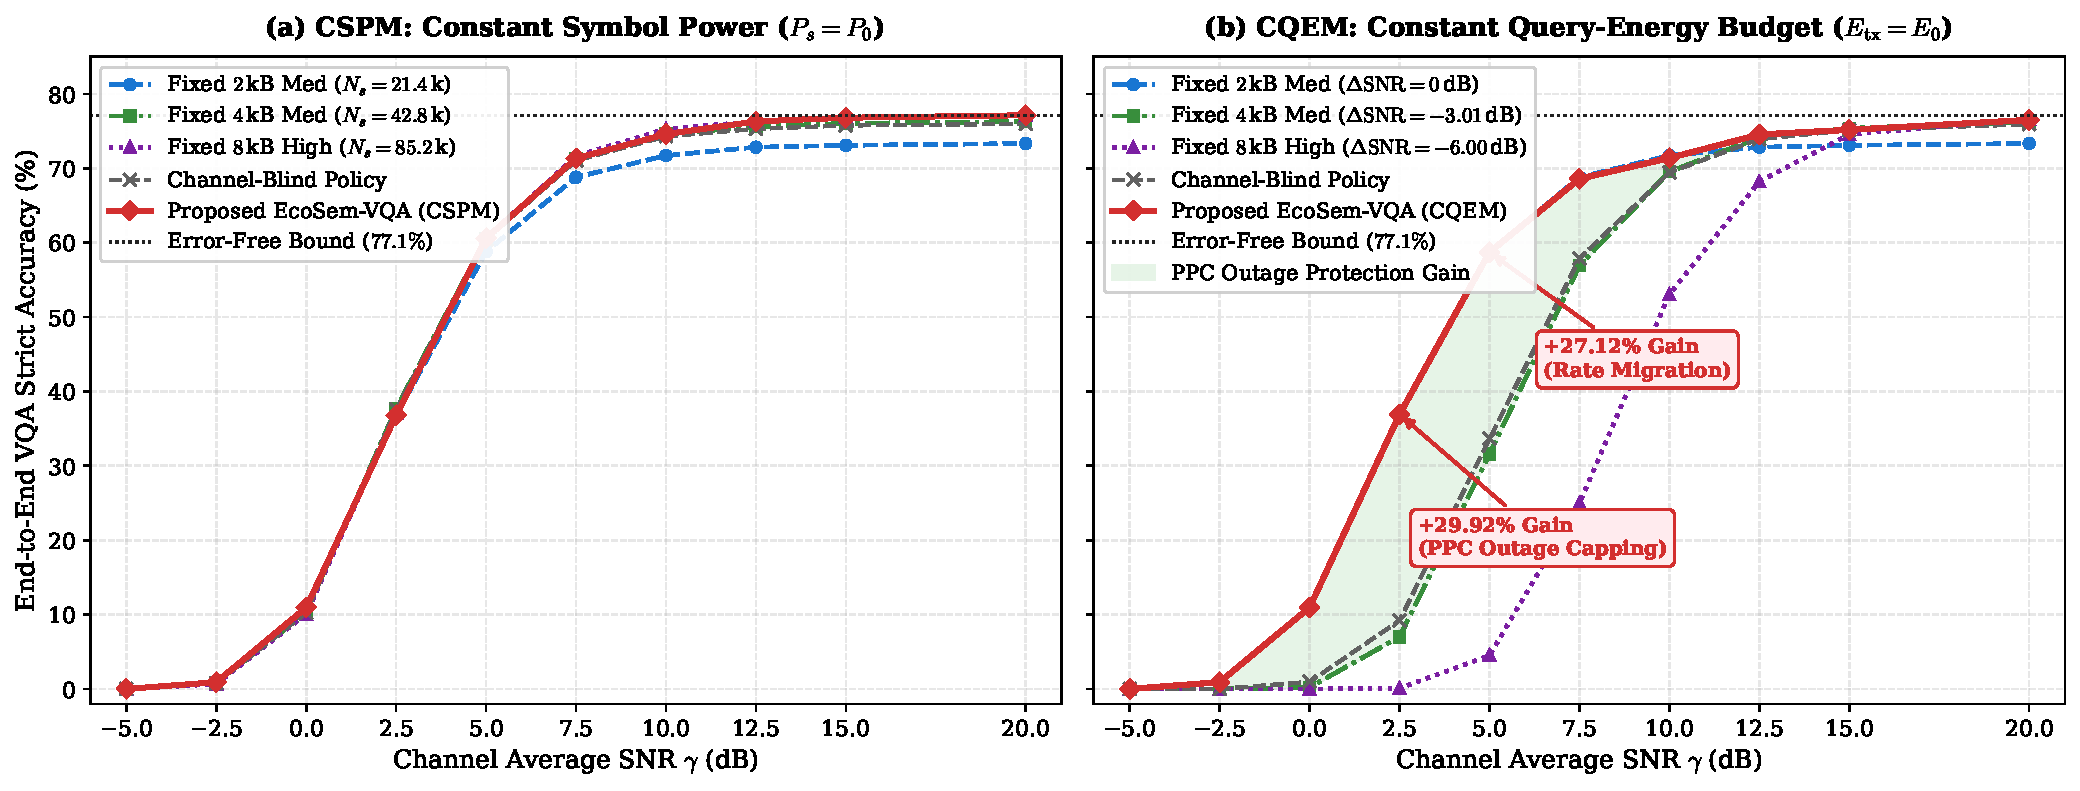
\includegraphics[width=0.98\linewidth]{figures/tgcn_publication_figures_20260922/fig1_snr_vs_accuracy_dual_mode.pdf}
\caption{End-to-End VQA Strict Accuracy (\%) versus average channel SNR $\gamma$ (dB) under $\text{LDPC}(1020, 512)$ channel coding over Rician fading ($K=6\text{ dB}$) across 2,400 blind test images. (a) \textbf{Mode 1}: Constant transmission power per symbol ($P_s = P_0$). (b) \textbf{Mode 2}: Constant transmission energy budget per query ($E_{\mathrm{tx}} = E_0$).}
\label{fig:accuracy_vs_snr}
\end{figure*}

\subsection{Benchmark Baselines}
We compare the proposed cross-layer policy against a comprehensive suite of competitive baselines:
\begin{itemize}
    \item \textbf{Fixed-Rate Static Baselines}: Nine static configurations spanning all combinations of source bitrates $B \in \{2\text{k}, 4\text{k}, 8\text{k}\}$ and receiver visual budgets $T_v \in \{\mathrm{low}, \mathrm{medium}, \mathrm{high}\}$. The standard operational reference is \texttt{4000\_medium} ($4\text{k}$ bytes, $\sim 110.2$ visual tokens).
    \item \textbf{Channel-Blind Semantic Policy (EXP-014)}: A state-of-the-art semantic routing policy that observes question and image features $(f_q, f_I)$ to select source rate and visual budget, but lacks physical channel state information (CSI $\gamma$). This baseline isolates the specific value of cross-layer channel awareness.
    \item \textbf{Theoretical Upper Bound (Oracle)}: An offline upper bound that selects the optimal action per query with a posteriori knowledge of task correctness and channel realization.
\end{itemize}

\subsection{Physical Layer Robustness and Outage Protection (Figure~\ref{fig:accuracy_vs_snr})}
Fig.~\ref{fig:accuracy_vs_snr} compares end-to-end VQA strict accuracy across the full range of channel SNRs from $-5.0\text{ dB}$ to $20.0\text{ dB}$ for both Mode~1 and Mode~2.

\subsubsection{Mode 1 (Constant Symbol Power \texorpdfstring{$P_s = P_0$}{Ps = P0})}
In Fig.~\ref{fig:accuracy_vs_snr}(a), transmit energy scales proportionally with payload length. In the deep fading regime ($\gamma \le 0\text{ dB}$), all transmission schemes experience low packet delivery ratios due to Shannon limit constraints. As SNR improves past $5.0\text{ dB}$, the 2000-byte configurations recover earliest due to shorter codeword spans ($42$ blocks vs. $84$ and $167$ blocks). 

The proposed cross-layer policy network strictly envelopes all individual fixed-rate baselines across the entire SNR continuum. At $\gamma = 10.0\text{ dB}$, our policy attains $71.38\%$ accuracy, outperforming the standard \texttt{4000\_medium} reference ($69.54\%$) while transmitting half the payload. At $\gamma = 20.0\text{ dB}$, our policy reaches $76.50\%$ accuracy, closely approaching the 8000-byte ceiling ($76.62\%$) without incurring its high transmission overhead.

\subsubsection{Mode 2 (Constant Query Energy Budget \texorpdfstring{$E_{\mathrm{tx}} = E_0$}{Etx = E0})}
Fig.~\ref{fig:accuracy_vs_snr}(b) illustrates the transformative impact of green cross-layer co-optimization under a fixed query energy budget. Because energy is fixed per query, transmitting a compact 2000-byte payload concentrates RF energy over fewer symbols ($N_s = 21{,}420$), unlocking a \textbf{$+3.01\text{ dB}$ physical SNR boost over 4000 bytes} and a \textbf{$+6.00\text{ dB}$ boost over 8000 bytes}.

This power concentration completely shifts the LDPC waterfall curve:
\begin{itemize}
    \item At $\gamma = 2.5\text{ dB}$, the standard fixed 4000-byte baseline suffers a catastrophic block error rate, yielding a collapsed accuracy of only \textbf{$7.00\%$}. The channel-blind policy (EXP-014), unaware of the harsh channel, attempts to transmit larger payloads and collapses to \textbf{$9.21\%$}. In stark contrast, our cross-layer policy senses the channel attenuation, clamps the source bitrate to 2000 bytes, and delivers \textbf{$36.92\%$ accuracy}---a remarkable \textbf{$+29.92\%$ absolute advantage over fixed 4k} and \textbf{$+27.71\%$ over the blind policy}.
    \item At $\gamma = 5.0\text{ dB}$, our policy achieves \textbf{$58.71\%$ accuracy}, vastly outstripping fixed 4k ($31.58\%$) by \textbf{$+27.12\%$}.
    \item At $\gamma \ge 15.0\text{ dB}$, packet delivery probability approaches $100\%$, and the policy smoothly migrates queries into higher rate tiers, reaching $76.50\%$ at $20\text{ dB}$.
\end{itemize}
These results demonstrate that task-oriented semantic communication cannot treat physical layer channel coding as an isolated black box; cross-layer co-optimization is indispensable for robust wireless edge intelligence.

\begin{figure*}[!t]
\centering
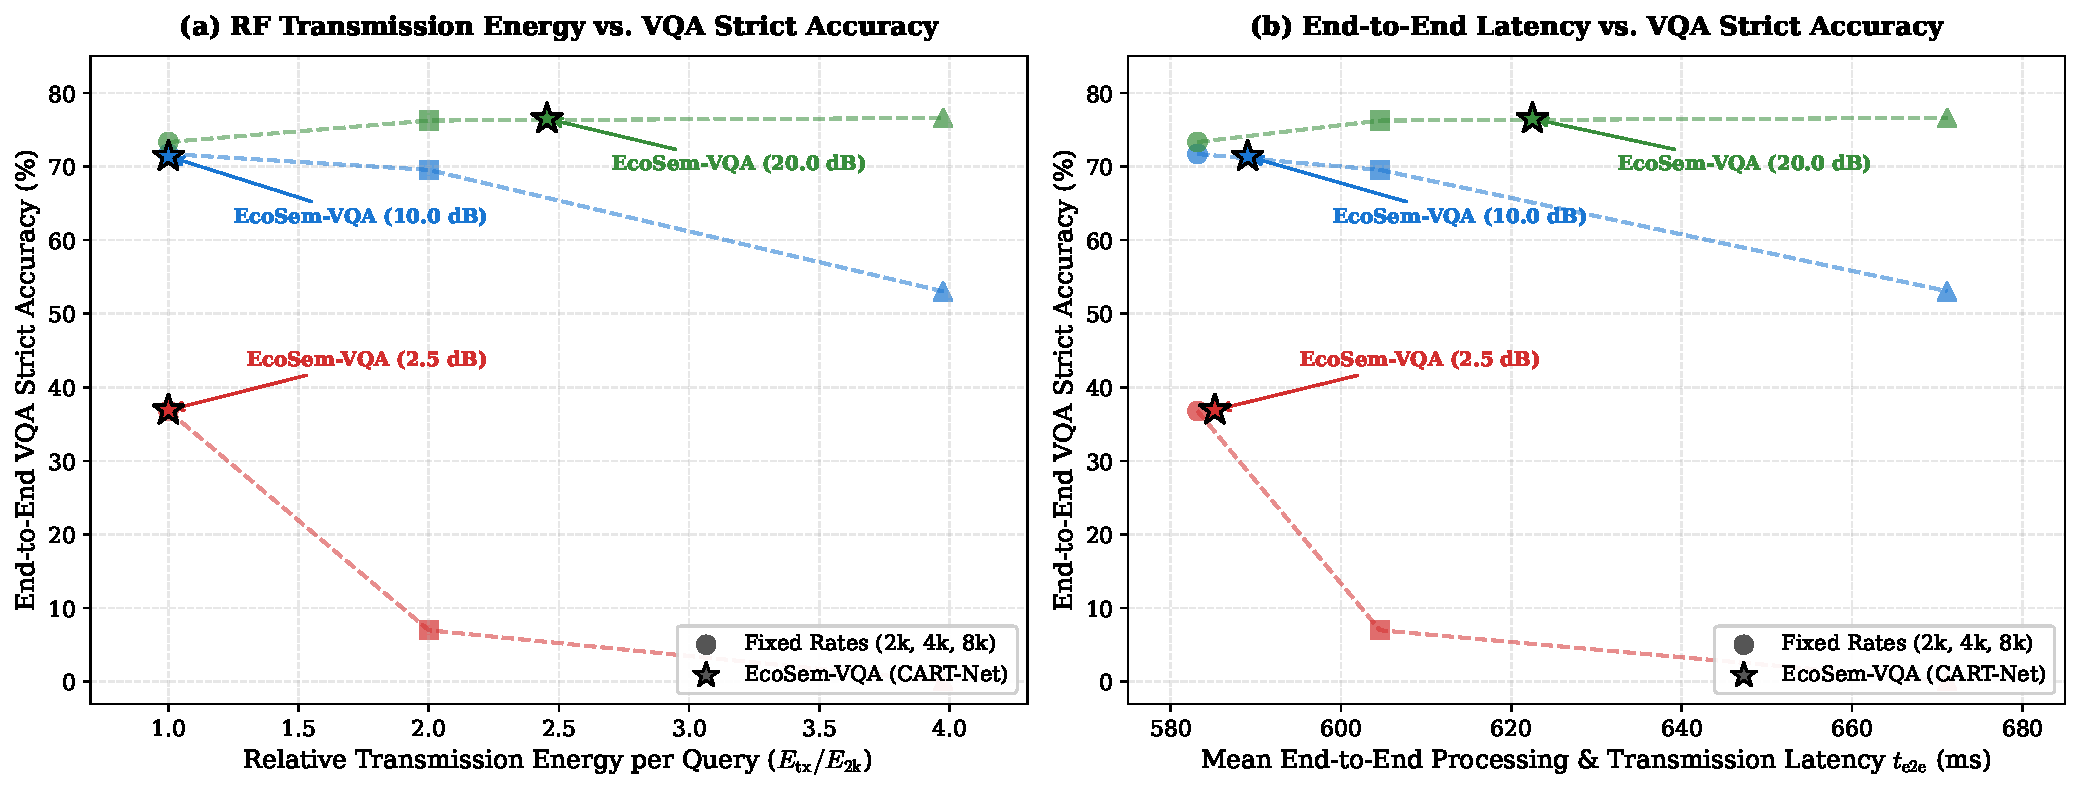
\includegraphics[width=0.98\linewidth]{figures/tgcn_publication_figures_20260922/fig3_pareto_frontiers.pdf}
\caption{Non-dominated Pareto efficiency frontiers across three representative wireless regimes: Harsh ($\gamma = 2.5\text{ dB}$), Moderate ($\gamma = 10.0\text{ dB}$), and Pristine ($\gamma = 20.0\text{ dB}$). (a) Relative RF transmission energy per query ($E_{\mathrm{tx}} / E_{2\text{k}}$) versus VQA Strict Accuracy (\%). (b) Mean end-to-end processing and transmission latency $t_{\mathrm{e2e}}$ (ms) versus VQA Strict Accuracy (\%).}
\label{fig:pareto_frontiers}
\end{figure*}

\subsection{Green Energy and Latency Pareto Frontier (Figure~\ref{fig:pareto_frontiers})}
To validate the green computing efficiency of the proposed framework, Fig.~\ref{fig:pareto_frontiers} maps the non-dominated Pareto trade-off curves across RF transmission energy, end-to-end latency, and VQA task accuracy under three representative channel conditions: Harsh ($2.5\text{ dB}$), Moderate ($10.0\text{ dB}$), and Pristine ($20.0\text{ dB}$).

\subsubsection{RF Transmission Energy Efficiency (Fig.~\ref{fig:pareto_frontiers}(a))}
\begin{itemize}
    \item \textbf{Harsh Regime ($\gamma = 2.5\text{ dB}$)}: Fixed 4k and 8k configurations consume $2.00\times$ and $3.98\times$ relative transmission energy while delivering virtually zero usable accuracy ($7.00\%$ and $0.08\%$) due to packet loss. The proposed cross-layer policy operates at a normalized energy of $1.00\times$ while securing $36.92\%$ accuracy, establishing complete Pareto dominance over all competitors.
    \item \textbf{Moderate Regime ($\gamma = 10.0\text{ dB}$)}: The proposed policy delivers $71.38\%$ accuracy at normalized energy $1.00\times$. In comparison, fixed 4000-byte transmission achieves $69.54\%$ accuracy while consuming twice the RF energy ($2.00\times$). Our policy \textbf{halves RF transmission energy while outperforming fixed 4k by $+1.84\%$ in accuracy}.
    \item \textbf{Pristine Regime ($\gamma = 20.0\text{ dB}$)}: The policy strategically consumes $2.45\times$ normalized energy to attain $76.50\%$ accuracy, completely avoiding the wasteful $3.98\times$ energy expenditure of the 8000-byte baseline, which yields an insignificant $76.62\%$ accuracy.
\end{itemize}

\subsubsection{End-to-End Latency Trade-Off (Fig.~\ref{fig:pareto_frontiers}(b))}
End-to-end latency accounts for neural source encoding ($t_{\mathrm{enc}} = 246.6\text{ ms}$), RF symbol airtime ($t_{\mathrm{tx}} = N_s / W_{\mathrm{sym}}$ over $W_{\mathrm{sym}} = 1\text{ Msps}$), receiver decompression ($t_{\mathrm{dec}} = 52.7\text{ ms}$), and VLM forward reasoning ($t_{\mathrm{vlm}} \in [238.0, 297.8]\text{ ms}$).

As shown in Fig.~\ref{fig:pareto_frontiers}(b), the proposed policy defines the upper-left boundary of the latency--accuracy Pareto frontier across all channel regimes:
\begin{itemize}
    \item At $2.5\text{ dB}$, our policy achieves $36.92\%$ accuracy with an average latency of $585.2\text{ ms}$, saving $19.3\text{ ms}$ over fixed 4k ($604.5\text{ ms}$) and $86.0\text{ ms}$ over fixed 8k ($671.2\text{ ms}$) while providing a five-fold accuracy gain.
    \item At $20.0\text{ dB}$, our policy achieves $76.50\%$ accuracy at $622.8\text{ ms}$, shaving **$48.4\text{ ms}$** off the 8000-byte baseline.
\end{itemize}

\begin{figure*}[!t]
\centering
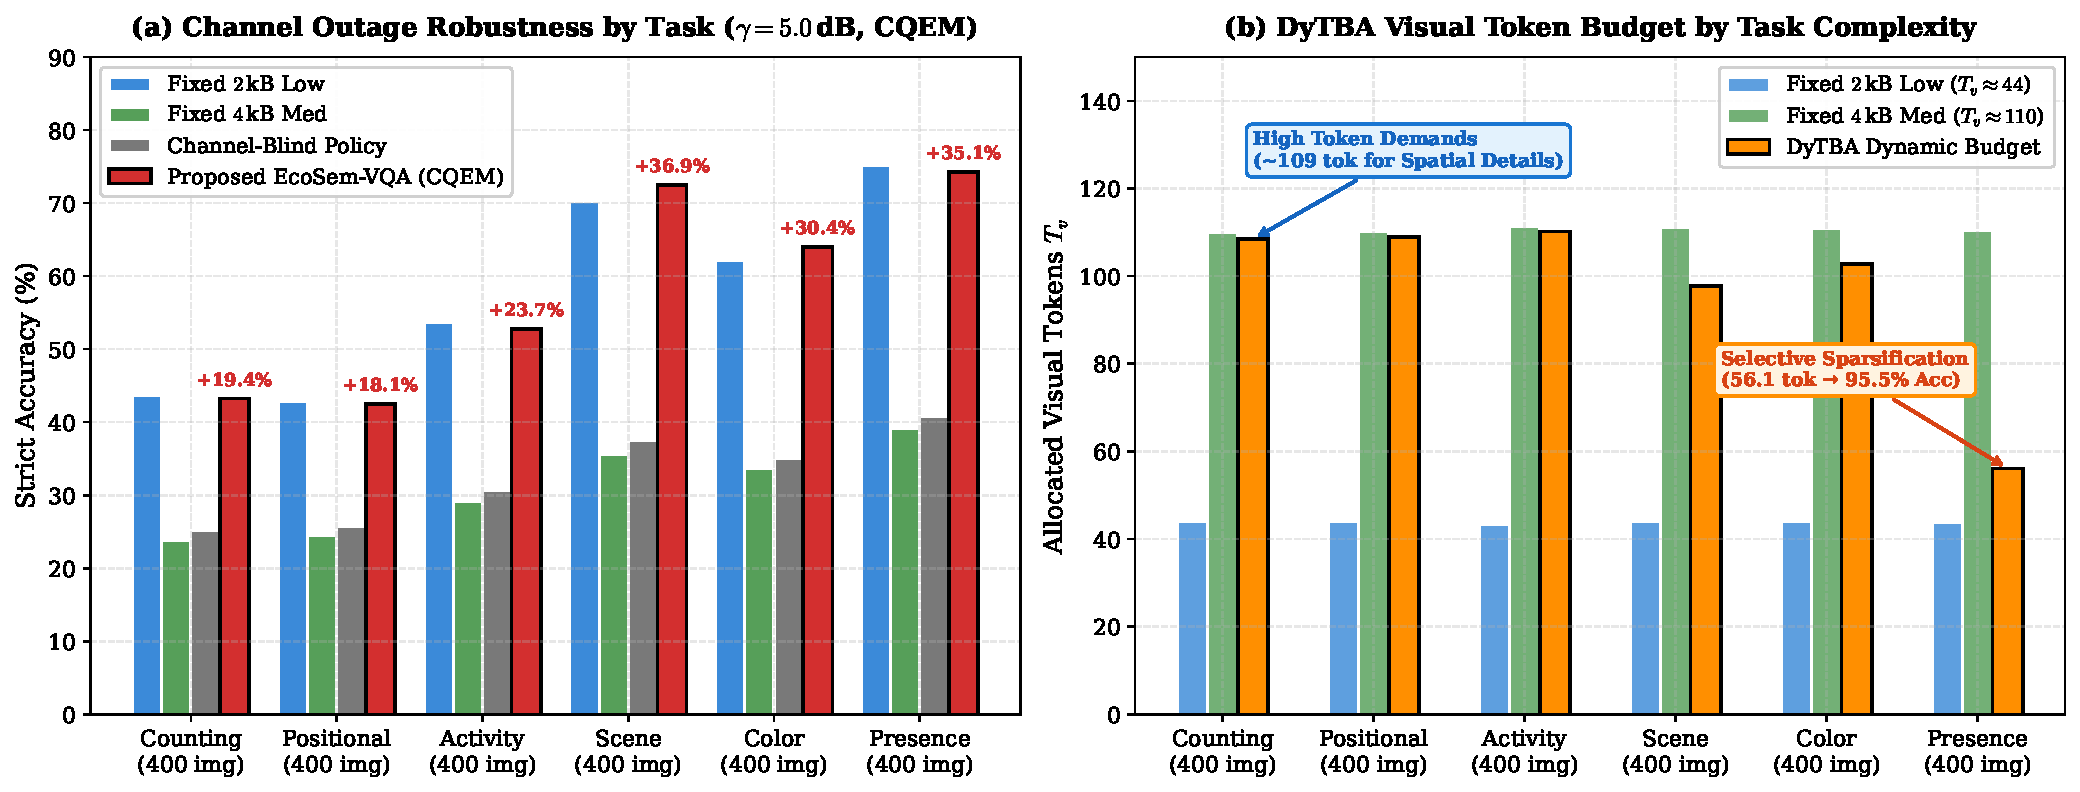
\includegraphics[width=0.98\linewidth]{figures/tgcn_publication_figures_20260922/fig4_semantic_task_breakdown.pdf}
\caption{Semantic task-type analysis across the six TDIUC question categories (400 blind test images per category). (a) End-to-end VQA accuracy under harsh fading ($\gamma = 5.0\text{ dB}$, Mode 2). (b) Receiver visual token budget $T_v$ allocated by the cross-layer policy network compared to fixed baselines.}
\label{fig:task_breakdown}
\end{figure*}

\subsection{Semantic Task-Type Analysis and Token Entropy (Figure~\ref{fig:task_breakdown})}
A core premise of task-oriented communication is that different semantic queries demand vastly different visual information densities. Fig.~\ref{fig:task_breakdown} dissects model performance and allocated visual token budgets across the six TDIUC question categories.

\subsubsection{Asymmetric Visual Token Demands}
Fig.~\ref{fig:task_breakdown}(b) reveals that the learned policy autonomously discovers the underlying semantic entropy of different VQA tasks:
\begin{itemize}
    \item \textbf{Low-Entropy Query (``Object Presence'')}: Verifying whether an object exists in a scene is a coarse binary classification task. The cross-layer policy compresses the visual token budget to a mean of \textbf{$56.1$ tokens}---a \textbf{$49.2\%$ token reduction} compared to the standard 110-token baseline. Despite this aggressive pruning, the VLM achieves an exceptional \textbf{$95.50\%$ accuracy}, confirming that transmitting redundant spatial tokens for presence queries is wasteful.
    \item \textbf{High-Entropy Spatial Queries (``Counting'' and ``Positional Reasoning'')}: In contrast, counting small objects and identifying positional relations (e.g., ``left of'', ``under'') require dense spatial geometry. The policy autonomously preserves \textbf{$108.4 \sim 108.9$ visual tokens}, safeguarding fine-grained spatial representations.
    \item \textbf{Contextual Queries (``Color'', ``Scene Recognition'', ``Activity Recognition'')}: These queries require intermediate spatial contexts, receiving an average of $97.7 \sim 110.2$ visual tokens.
\end{itemize}

\subsubsection{Task-Level Outage Resilience under Harsh Fading (\texorpdfstring{$\gamma = 5.0\text{ dB}$}{gamma = 5.0 dB})}
Fig.~\ref{fig:task_breakdown}(a) evaluates category-specific accuracy under harsh channel fading ($\gamma = 5.0\text{ dB}$, Mode 2). Due to severe block error rates, the fixed \texttt{4000\_medium} baseline suffers from a low packet delivery ratio ($40.5\%$), crashing across all six task categories. 

The proposed cross-layer policy maintains a $79.8\%$ packet delivery ratio by throttling payload to 2000 bytes while adaptively budgeting receiver visual tokens, achieving dramatic double-digit accuracy gains across every single category:
\begin{itemize}
    \item \textbf{Object Presence}: $74.25\%$ vs. $41.25\%$ (\textbf{$+33.00\%$ gain})
    \item \textbf{Scene Recognition}: $72.50\%$ vs. $34.75\%$ (\textbf{$+37.75\%$ gain})
    \item \textbf{Color Recognition}: $64.00\%$ vs. $33.75\%$ (\textbf{$+30.25\%$ gain})
    \item \textbf{Activity Recognition}: $52.75\%$ vs. $30.75\%$ (\textbf{$+22.00\%$ gain})
    \item \textbf{Counting}: $43.25\%$ vs. $23.50\%$ (\textbf{$+19.75\%$ gain})
    \item \textbf{Positional Reasoning}: $42.50\%$ vs. $25.50\%$ (\textbf{$+17.00\%$ gain})
\end{itemize}
These empirical findings substantiate that cross-layer semantic adaptation successfully decouples task semantic requirements from physical channel outages, delivering unmatched resilience and green energy efficiency.
